\chapter{Results and discussion}
\section{Number of simulations}

The  algorithm makes usage of randomly distributed users causing each simulation to be difference. The results are based on average 
values over multiple simulations. It is therefore important knowing how mush simulations is required in order to become a converged average.
This is done by using an example scenario which details can be found in table \ref{table:configForNumberOfUsers}. The most important parameters
investigated in the different scenarios are $SAR_{10g}$, power consumption and user coverage. Therefore, the cummulative avarage of each investigated 
value is plotted in function of number of simulations.

\begin{table}[!htb]
\centering
  \begin{tabular}{|l|l|}
  \hline
  Parameter               & value          \\   \hline 
  number of users               & 40            \\ 
  facilityCapacity                    & 20           \\ 
  fixedFlyHeight               & 100           \\ 
  optimization strategy               & power consumption optimized           \\ 
  \hline
  \end{tabular}
  \caption{Overview of the configuration.}
  \label{table:confOverviewScenario2}
\end{table}

The number of simulations has a direct influence on the runtime. Certain configurations take a considerable amount of runtime (expessed in hours). This is because of the
exponential time complexity. The deployment tool with $n$ users, will need to calculate $n$ times the pathloss between $n$ drones and $n$ users and thereafter $n/2$ times between
each user. Thereafter, each user will have to be connected to the best possible \gls{UABS} and each user is therefore required to consider multiple \gls{UABS}s.

\begin{figure}[th!]
  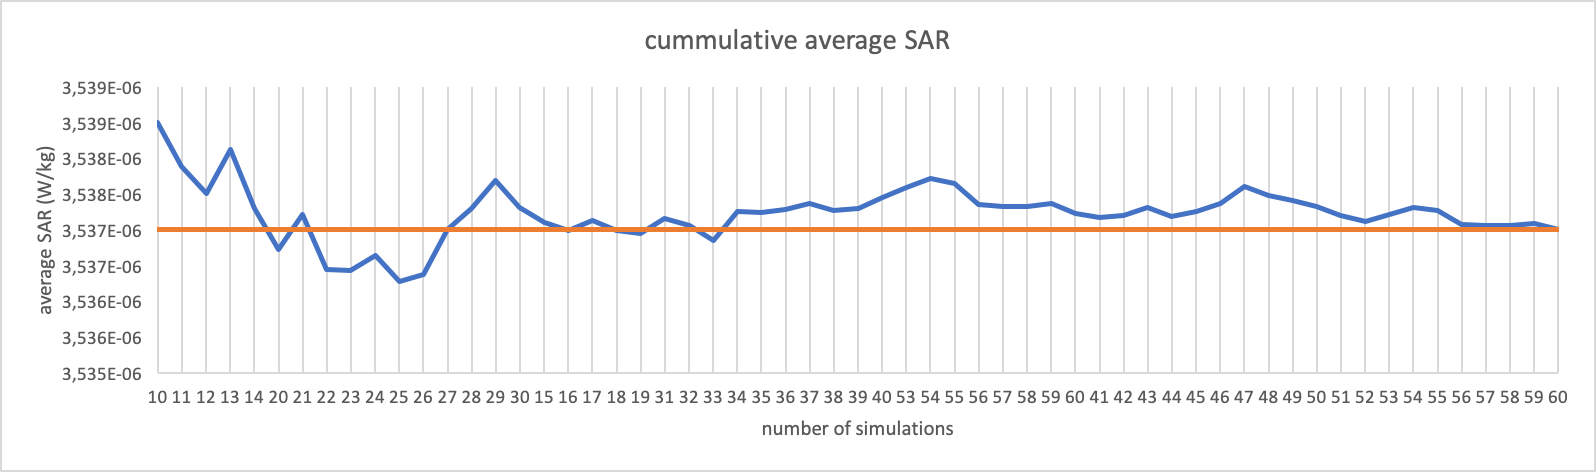
\includegraphics[width=\textwidth]{../results/numberOfSim/sarvssim.png}
  \caption{General design of a microstrip antenna}
  \label{fig:fhsar}
\end{figure}
\begin{figure}[th!]
  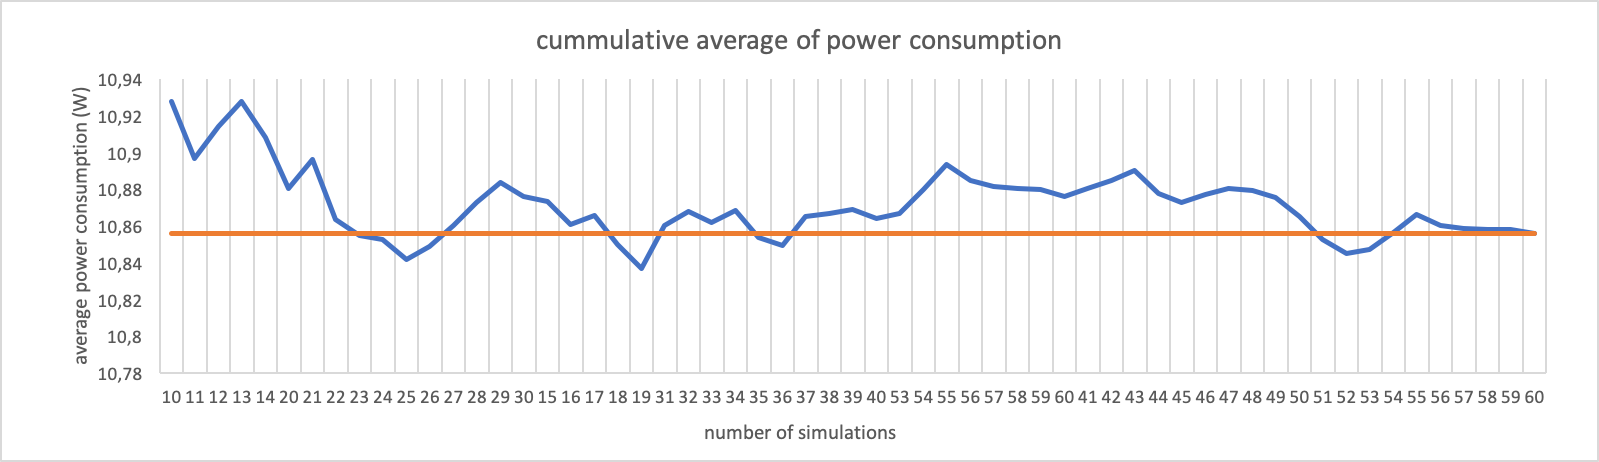
\includegraphics[width=\textwidth]{../results/numberOfSim/pcvssim.png}
  \caption{General design of a microstrip antenna}
  \label{fig:fhsar}
\end{figure}
\begin{figure}[th!]
  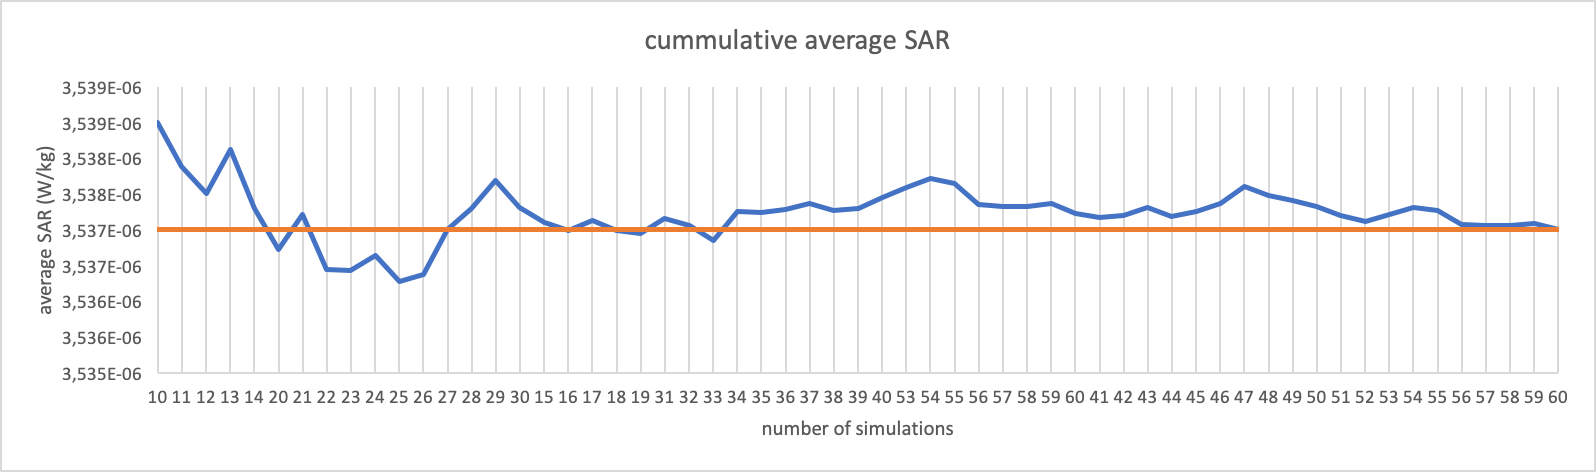
\includegraphics[width=\textwidth]{../results/numberOfSim/sarvssim.png}
  \caption{General design of a microstrip antenna}
  \label{fig:fhsar}
\end{figure}

\section{Scenario 1: one user and one basestation}


\subsection{The influence of the fly height on $SAR_{10g}$}
\label{sub:senario1_influenceOfFlyHeight}

This section investigates how the fly height of the \gls{UABS} influence $SAR_{10g}$ and power consumption. In figure \ref{fig:fhsar}
becomes clear that with an increasing flyheight, the specific absorption rate grows exponentially which is also the case for the power consumption (fig. \ref{fig:pcsar})  

This behavior has been examined for the two types of antennae which are the fictional \gls{isotropicradiator} and the microstrip patch antenna. In figures 
\ref{fig:fhsar} and \ref{fig:pcsar} becomes clear that the type of antenna does not influence the power consumption nor the specific absorption rate in this  scenario.
The reasoning behind this is that the tool will possition the \gls{UABS} just above the user. An \gls{isotropicradiator} doesn't experience attenuation while a microstrip
patch antenna does. The later is however pointing to the ground meaning the user is in the perfect center of the main beam and therefore also
not experiencing any attenuation from the normalized radiation pattern.

The deployment tool will only place a drone if the possition is feasable meaning that if the user is inside a building which is higher then
the fly height of the drone, no \gls{UABS} would be place. In normal circumstances, with more \gls{UABS}s, annother nearby drone would try to 
take over the responsibility. However, since only one drone is available in this scenario, the user would remain uncovered. To make sure only covered users
are considered in this scenario, the user in question will always be located in the same outdoor location. The location chosen for this situation is longitude 3.73311°E and 
latitude  51.05992°N.

\begin{figure}[th!]
  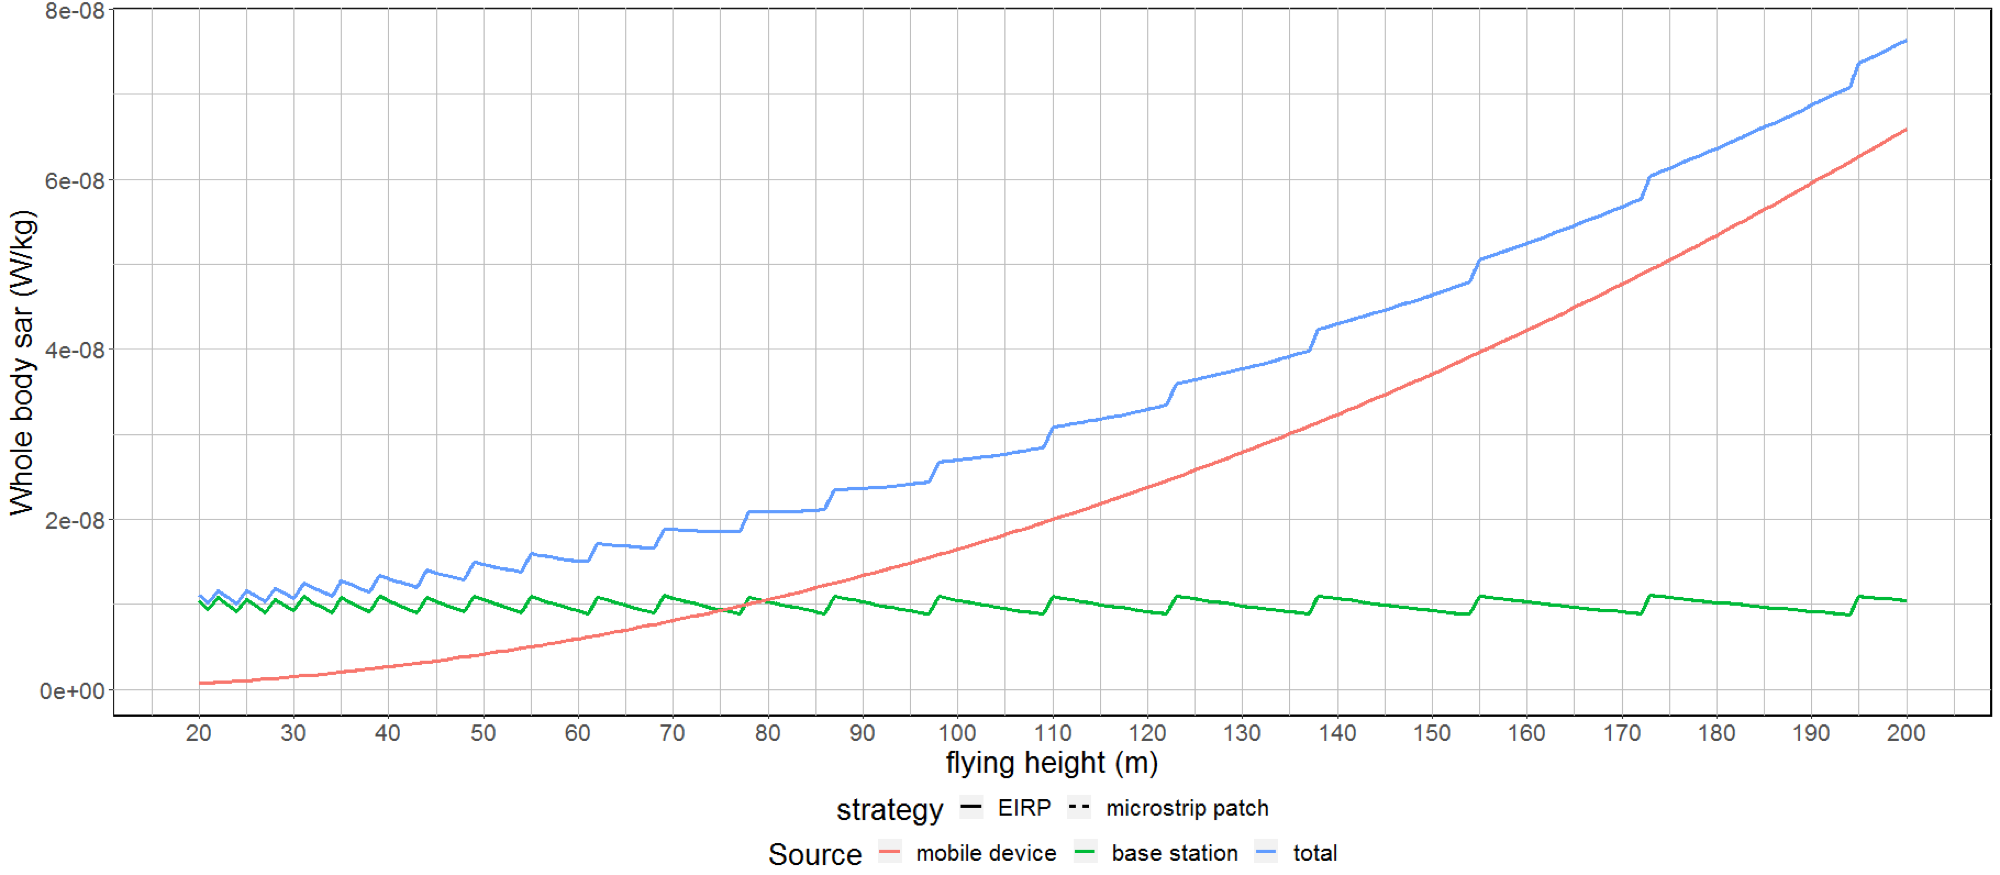
\includegraphics[width=\textwidth]{../results/s1/flyheight-sar.png}
  \caption{General design of a microstrip antenna}
  \label{fig:fhsar}
\end{figure}

\begin{figure}[bh!]
  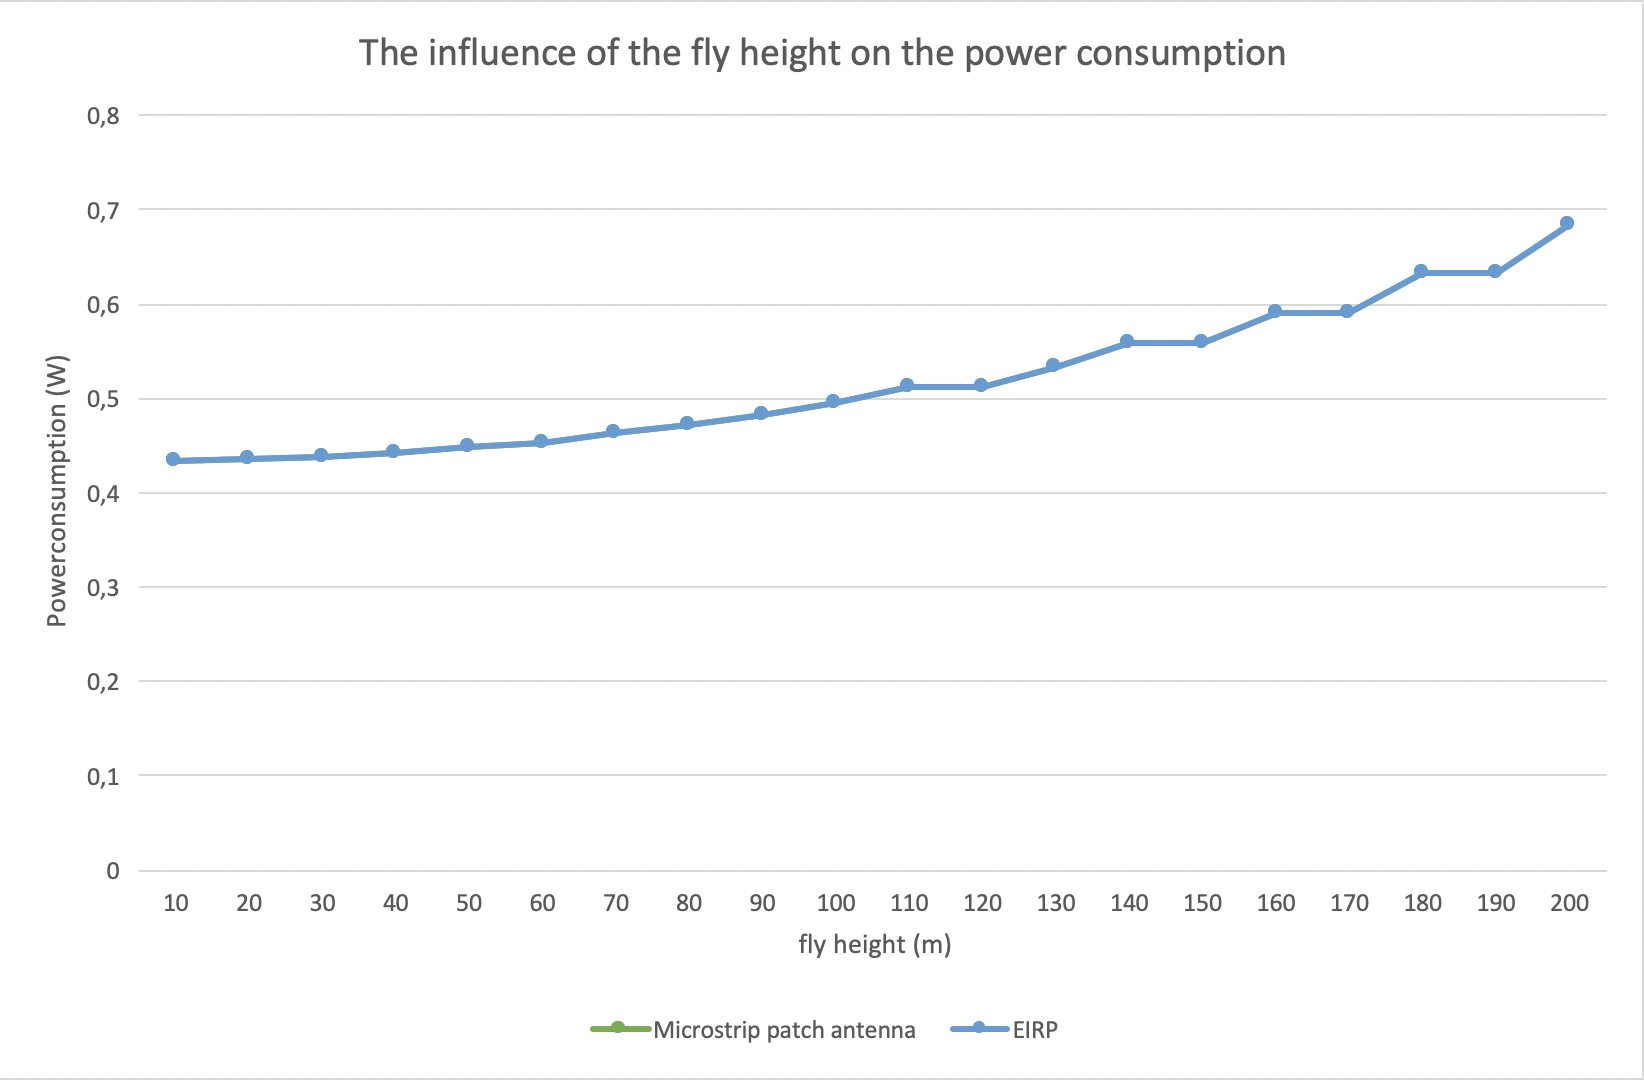
\includegraphics[width=\textwidth]{../results/s1/flyheight-pc.png}
  \caption{General design of a microstrip antenna}
  \label{fig:pcsar}
\end{figure}

\subsection{The influence from the maximum transmission power}
\gls{LTE} makes usages of power control meaning that no more power will be used then strictly necessary. The actual 
transmit power $P_{tx}$ therefore ranges between 0 and the maximum input power. $P_{tx}$ is zero when either no user is 
present or the user is so far away that the actual tranmit power would exceed the maximum transmission power.

Increasing the maximum tranmission power won't influence the power consumption or $SAR_{10g}$ because the \gls{UABS} won't use more
then strictly required. It is therefore more usefull to match the transmission power against a variable fly height. Figure \ref{fig:ptxfh}
shows a logarithmic  relationship showing that $P_{tx}$ increases fast at low altitude but slows down at lower altitudes. 

Since it became clear from section \ref{sub:senario1_influenceOfFlyHeight} that the type of antenna won't make a difference when applying
the tool in this scenario, it is not usefull to repeat this test with different types of antennae.


\begin{figure}[h!]
  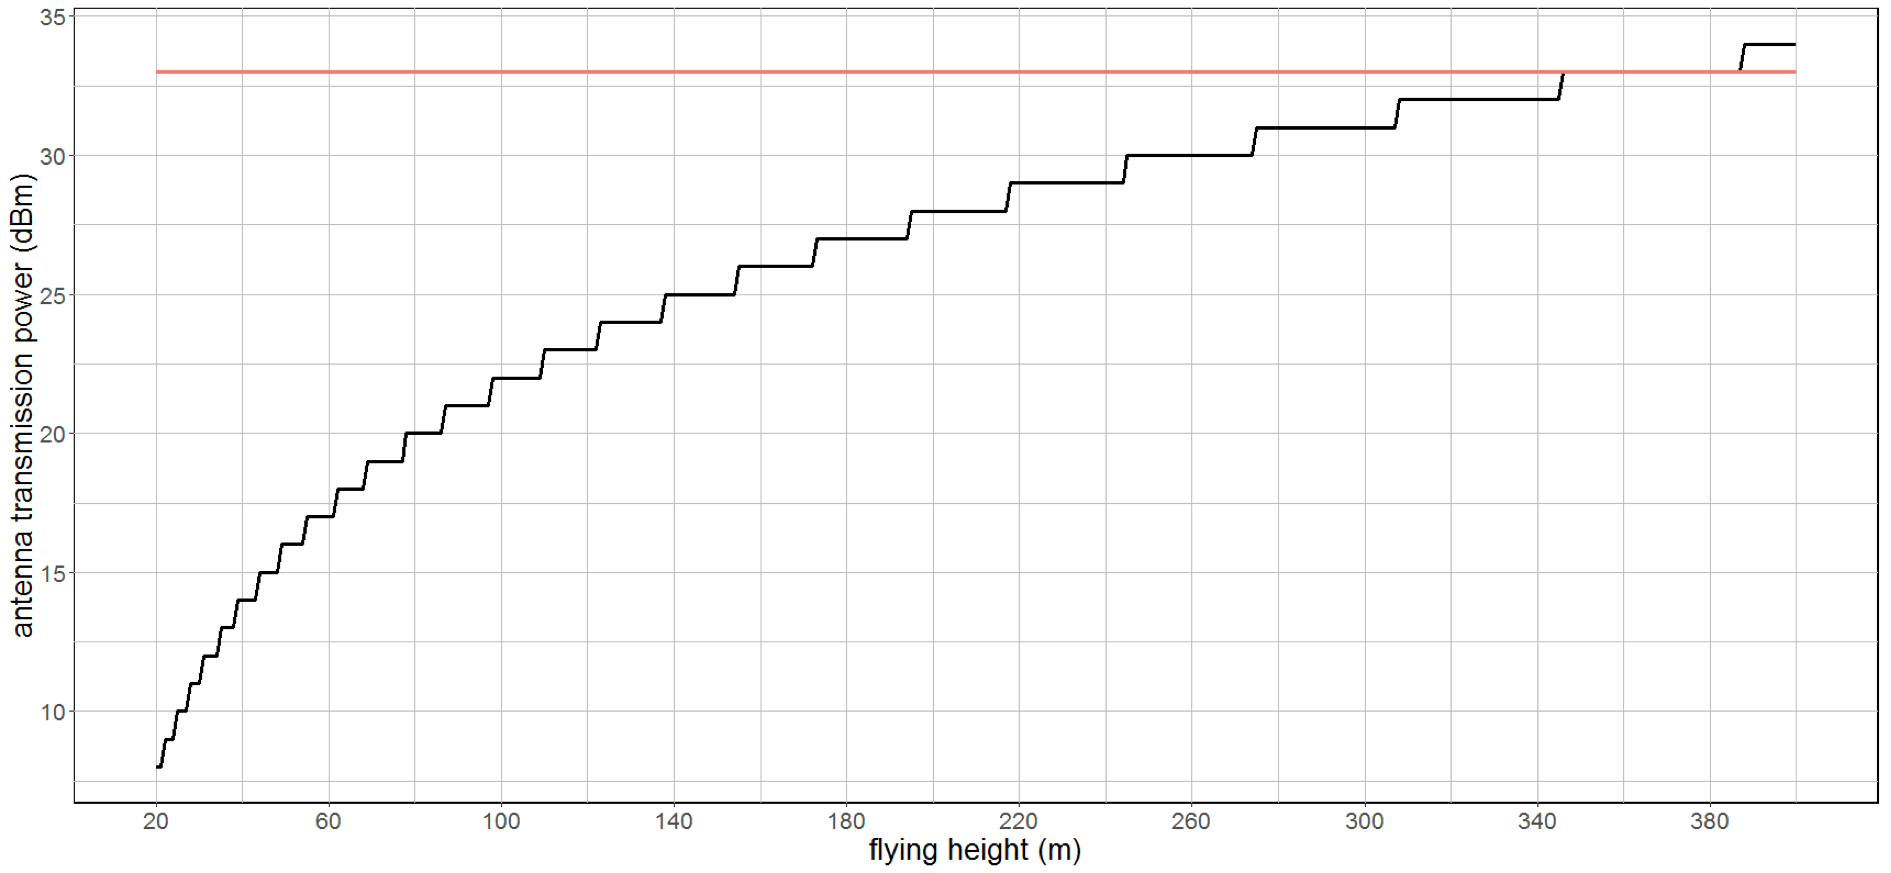
\includegraphics[width=\textwidth]{../results/s1/ptx-fh.png}
  \caption{General design of a microstrip antenna}
  \label{fig:ptxfh}
\end{figure}

\section{Scenario 2: increased traffic}

\subsection{Influence of the flight altitude}
The first case of this scenario investigates the influ

\section{Scenario 3:}